\section{Model przypadków użycia}

\subsection{Diagram pakietów przypadków użycia}

Jednym z głównych elementów prac projektowych było wykonanie diagramu przypadków użycia. Zgodnie z definicją diagram taki składa się z przypadków użycia, czyli jednostek funkcjonalności dostarczanych przez system, które są realizowane jako ciąg interakcji pomiędzy aktorem a systemem \cite{usecase}. Z tego względu, że w wyniku prac projektowych powstał diagram o bardzo dużej liczbie przypadków użycia, zdecydowano podzielić się go na składowe i utworzyć na podstawie tych składowych diagram pakietów przypadków użycia. 

Według materiałów opisujących metodykę RUP \cite{caseuse} - pakiet przypadków użycia jest zbiorem przypadków użycia, aktorów, relacji, diagramów i innych pakietów. Najczęstsze jego zastosowanie to próba restrukturyzacji diagramu przypadków użycia poprzez podzielenie go na składowe. W projektowanym systemie również został do tego wykorzystany. Skutkiem tego było utworzenie kilku, przedstawionych poniżej pakietów przypadków użycia(Rys. \ref{chapter4_package}):


\begin{figure}[ht]
	\centering
	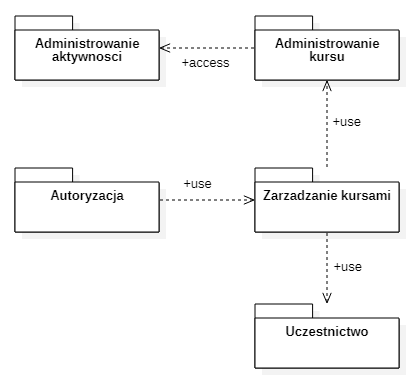
\includegraphics[scale=0.9]{img/chapter4/package_diagram.png}
	\caption{Diagram pakietów przypadków użycia}
	\label{chapter4_package}
\end{figure}

Rozbicie diagramu na pakiety pozwala na podzielenie procesu tworzenia aplikacji na kilka jednostek czasu. Takie okresy uzyskały przypisany do siebie zestaw przypadków użycia, które wymagają implementacji w jego trakcie. W pierwszej kolejności skupiono się na pakietach autoryzacja oraz zarządzanie kursami, co stanowi solidną podstawę i zapewnia możliwość szybkiej implementacji pozostałych pakietów. 

\subsection{Diagramy przypadków użycia}


Podczas prac projektowych powstało 5 podstawowych pakietów przypadków użycia. Aktorzy oraz przypadki użycia wchodzące w ich skład zostały one opisane w tabelach poniżej. Autoryzacja to pakiet obejmujący swoim zakresem wszystkie przypadki użycia związane z zakładaniem konta, logowaniem czy ustawieniami konta i jest na tyle podstawowym przykładem zbioru przypadków użycia iż nie został tutaj szczegółowo opisany. Drugim z pakietów przypadków użycia jest pakiet zarządzania kursami. W jego skład wchodzi jeden aktor (użytkownik) oraz przypadki użycia, które determinują sytuacje, w których użytkownik ma do czynienia z zapisywaniem i tworzeniem kursów (Rys.  \ref{chapter4_zarzadzanie_kurs})